\documentclass[12pt]{article}
\usepackage[utf8]{inputenc}
\usepackage{authblk}
\usepackage{graphicx} % Lib de importar e tratar imagem
\usepackage[english,brazil]{babel} % Manter dois idiomas
\usepackage{fancyhdr} % Configuração das paginas
\usepackage{float}
\usepackage{xcolor}
\usepackage{titlesec}
\usepackage{background} % Componente de Watermark
\usepackage{hyperref}
\usepackage{verbatim}
\usepackage{tcolorbox}
\usepackage[a4paper, left=2cm, right=2cm]{geometry}

\newcommand{\shellcmd}[1]{\\\indent\indent\texttt{\footnotesize\# #1}\\}

% Definir as características do hyperlink
\hypersetup{
    colorlinks=true,
    linkcolor=blue,
    filecolor=magenta,      
    urlcolor=cyan,
    pdftitle={Overleaf Example},
    pdfpagemode=FullScreen,
}

%Função para diminuir tamanho da fonte
\newcommand{\changefont}{%
    \fontsize{9}{12}\selectfont
}

%Document Layout Config
\pagestyle{fancy}
\setlength\headheight{26pt}
\setlength\parindent{0pt}
\fancyhf{}

% Header  Config
\fancyhead[RO]{New MySafe - Account Recovery}
\fancyhead[LO]{\includegraphics[width=0.7cm]{Logo.png}}

% Footer  Config
\renewcommand{\footrulewidth}{0.4pt} % Inserir linha no final da pagina "pre-footer"
\fancyfoot[RO]{\includegraphics[width=0.7cm]{Logo.png}}

%Document Specification
\title{New MySafe - Account Recovery}
\author{senhasegura}
\affil{Departamento de Segurança e Inovação - SEGi9}
\date{}
\graphicspath{ {img/} }

%Capa
\begin{document}
\NoBgThispage % Ignorar background na capa
\maketitle
\begin{center}

\includegraphics{logo.png}
\end{center}
\begin{center}
\textbf{\LARGE \\CONFIDENCIAL}
\end{center}
\pagenumbering{gobble} % Não contar como página a capa
\pagebreak

%Marca d'agua
\backgroundsetup{contents=
\includegraphics{logo.png}, scale=1.5, opacity=0.15, angle=0}

%Resumo Executivo
\section*{\centering{Resumo Executivo}}
\vspace*{\fill}
\large{Este texto aborda o processo de recuperação das chaves de criptografia dos Usuários, no qual o Custodiante designado restaura as chaves de criptografia dos usuários  de uma organização. Desta forma, o Custodiante restabelece o acesso em casos de esquecimento ou perda da senha mestra por parte dos Usuários. Essa funcionalidade pode ser ativada para a organização ao habilitar a política de administração de recuperação de chave de criptografia.}
\vspace*{\fill}
\fancyfoot[CO]{senhasegura\\ \changefont Qualquer reprodução ou distribuição é estritamente proibida sem a aprovação prévia por escrito da empresa MT4.}

\pagebreak

%Sumario
\tableofcontents

\pagebreak

%Rodapé
\fancyfoot[CO]{\thepage\\\changefont Qualquer reprodução ou distribuição é estritamente proibida sem a aprovação prévia por escrito da empresa MT4.}
\pagenumbering{arabic}

\textbf{Nota sobre os exemplos:} os comandos com AES-CBC abaixo ilustram a proteção de confidencialidade e deixam explícitos chave e IV. Em uma implementação real, cada texto cifrado deve também ser autenticado (por exemplo, com HMAC em chave independente) ou protegido por uma construção AEAD apropriada.

\pagebreak

% Página
\section{Segurança das Chaves de Criptografia}

\subsection{Alice}

Processo de criação das chaves, Pública (KPuAlice.pem), Privada (KPrAlice.pem) e de Dados (DEKAlice.bin), juntamente com o processo de encriptação para armazenamento seguro das chaves Privada (KPrAlice.pem) e de Dados (DEKAlice).

\begin{figure}[H]
	\centering
	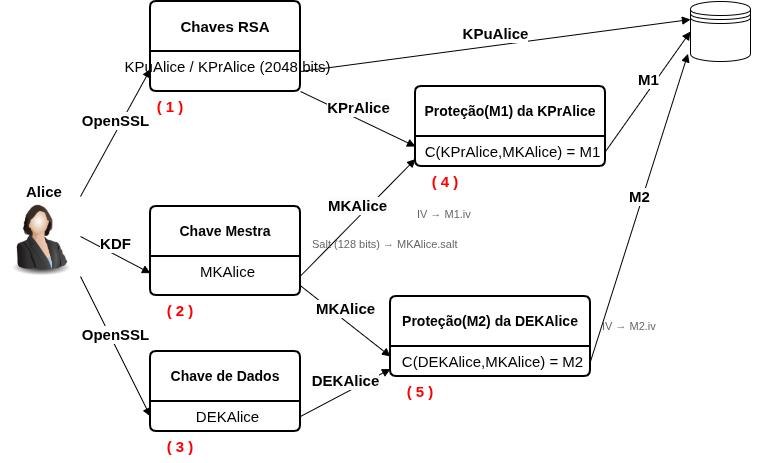
\includegraphics[scale=0.55]{chave_alice.png}
	\caption{Chaves e Processos associadas a Alice (M1 e M2: ver nota sobre autenticação)}
	\label{fig:chave_alice}
\end{figure}

\begin{enumerate}
	\item Criação da Chave Pública (KPuAlice.pem) e da Chave Privada (KPrAlice.pem);
	\begin{tcolorbox}[width=\textwidth]
		{\scriptsize
			\begin{verbatim}
			$ openssl genpkey -algorithm RSA -pkeyopt rsa_keygen_bits:2048 -out KPrAlice.pem
			$ openssl rsa -pubout -in KPrAlice.pem -out KPuAlice.pem
			$ openssl req -new -x509 -key KPrAlice.pem -out Alice.cert.pem \
			  -subj "/CN=Alice"
			\end{verbatim}
		}
	\end{tcolorbox}
	\item Derivação local da Chave Mestra da Alice (MKAlice.hex), baseada na Senha Mestra (MPAlice). O salt de 128 bits é armazenado separadamente para permitir a derivação durante a recuperação;
	\begin{tcolorbox}[width=\textwidth]
		{\scriptsize
			\begin{verbatim}
			$ read -rs MASTER_PASSWORD
			$ SALT_HEX=$(openssl rand -hex 16)
			$ printf '%s' "$SALT_HEX" > MKAlice.salt
			$ openssl kdf -keylen 32 -kdfopt digest:SHA256 \
			  -kdfopt pass:"$MASTER_PASSWORD" -kdfopt salt:"$SALT_HEX" \
			  -kdfopt iter:600000 PBKDF2 | tr -d ':\n' > MKAlice.hex
			\end{verbatim}
		}
	\end{tcolorbox}
	\item Criação da Chave de Dados (DEKAlice.bin);
	\begin{tcolorbox}[width=\textwidth]
		{\scriptsize
			\begin{verbatim}
			$ openssl rand -out DEKAlice.bin 32
			\end{verbatim}
		}
	\end{tcolorbox}
	\item A Chave Privada (KPrAlice.pem) é protegida com a Chave Mestra (MKAlice.hex), gerando o Texto Cifrado M1. O IV é armazenado junto com o artefato cifrado;
	\begin{tcolorbox}[width=\textwidth]
		{\scriptsize
			\begin{verbatim}
			$ IV_HEX=$(openssl rand -hex 16)
			$ printf '%s' "$IV_HEX" > M1.iv
			$ openssl enc -aes-256-cbc -K "$(cat MKAlice.hex)" -iv "$IV_HEX" \
			  -in KPrAlice.pem -out M1.bin
			\end{verbatim}
		}
	\end{tcolorbox}
	\item A Chave de Dados (DEKAlice.bin) é protegida com a Chave Mestra (MKAlice.hex), gerando o Texto Cifrado M2 que é enviado para o servidor.
	\begin{tcolorbox}[width=\textwidth]
		{\scriptsize
			\begin{verbatim}
			$ IV_HEX=$(openssl rand -hex 16)
			$ printf '%s' "$IV_HEX" > M2.iv
			$ openssl enc -aes-256-cbc -K "$(cat MKAlice.hex)" -iv "$IV_HEX" \
			  -in DEKAlice.bin -out M2.bin
			\end{verbatim}
		}
	\end{tcolorbox}
\end{enumerate}

\subsection{Bob}

Processo de criação das chaves, Pública (KPuBob.pem), Privada (KPrBob.pem) e de Dados (DEKBob.bin), juntamente com o processo de encriptação para armazenamento seguro das chaves Privada (KPrBob.pem) e de Dados (DEKBob.bin).

\begin{figure}[H]
	\centering
	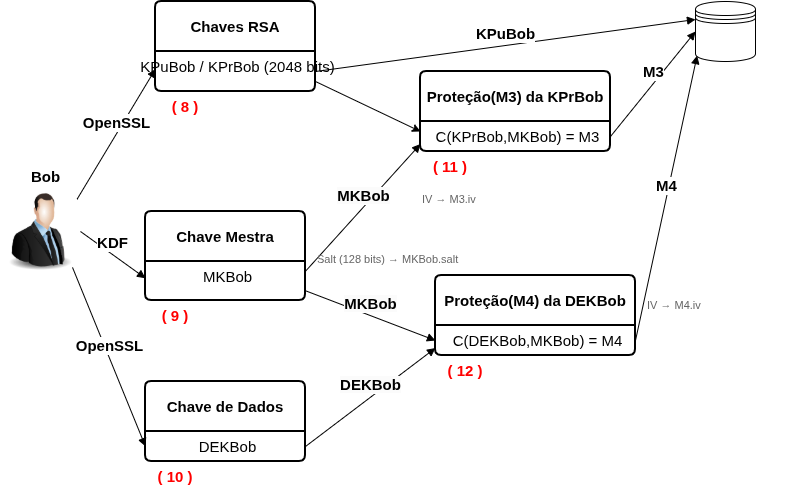
\includegraphics[scale=0.55]{chave_bob.png}
	\caption{Chaves e Processos associados ao Bob (M3 e M4: ver nota sobre autenticação)}
	\label{fig:chave_bob}
\end{figure}

\begin{enumerate}
	\setcounter{enumi}{7} % Define o contador para começar do número 8
		\item Criação das Chave Pública (KPuBob.pem) e da Chave Privada (KPrBob.pem);
		\begin{tcolorbox}[width=\textwidth]
			{\scriptsize
				\begin{verbatim}
				$ openssl genpkey -algorithm RSA -pkeyopt rsa_keygen_bits:2048 -out KPrBob.pem
				$ openssl rsa -pubout -in KPrBob.pem -out KPuBob.pem
				\end{verbatim}
			}
		\end{tcolorbox}
		\item Derivação local da Chave Mestra (MKBob.hex) baseada na Senha Mestra (MPBob);
		\begin{tcolorbox}[width=\textwidth]
			{\scriptsize
				\begin{verbatim}
					$ read -rs MASTER_PASSWORD
					$ SALT_HEX=$(openssl rand -hex 16)
					$ printf '%s' "$SALT_HEX" > MKBob.salt
					$ openssl kdf -keylen 32 -kdfopt digest:SHA256 \
					  -kdfopt pass:"$MASTER_PASSWORD" -kdfopt salt:"$SALT_HEX" \
					  -kdfopt iter:600000 PBKDF2 | tr -d ':\n' > MKBob.hex
				\end{verbatim}
			}
		\end{tcolorbox}
		\item Criação da Chave de Dados (DEKBob.bin);
		\begin{tcolorbox}[width=\textwidth]
			{\scriptsize
				\begin{verbatim}
				$ openssl rand -out DEKBob.bin 32
				\end{verbatim}
			}
		\end{tcolorbox}
		\item A Chave Privada (KPrBob) é protegida com a Chave Mestra (MKBob.hex), gerando o Texto Cifrado M3 que é enviado para o servidor;
		\begin{tcolorbox}[width=\textwidth]
			{\scriptsize
				\begin{verbatim}
				$ IV_HEX=$(openssl rand -hex 16)
				$ printf '%s' "$IV_HEX" > M3.iv
				$ openssl enc -aes-256-cbc -K "$(cat MKBob.hex)" -iv "$IV_HEX" \
				  -in KPrBob.pem -out M3.bin
				\end{verbatim}
			}
		\end{tcolorbox}
		\item A Chave de Dados (DEKBob.bin) é protegida com a Chave Mestra (MKBob.hex), gerando o Texto Cifrado M4 que é enviado para o servidor.
		\begin{tcolorbox}[width=\textwidth]
			{\scriptsize
				\begin{verbatim}
				$ IV_HEX=$(openssl rand -hex 16)
				$ printf '%s' "$IV_HEX" > M4.iv
				$ openssl enc -aes-256-cbc -K "$(cat MKBob.hex)" -iv "$IV_HEX" \
				  -in DEKBob.bin -out M4.bin
				\end{verbatim}
			}
		\end{tcolorbox}
\end{enumerate}

\pagebreak

% Página
\section{Custódia das Chaves de Criptografia}

No exemplo apresentado, Alice é a usuária Custodiante e Bob é o usuário que terá as suas chaves custodiadas. Assim, todas as chaves do Bob devem ser compartilhadas com a Custodiante Alice.

\subsection{Custodiando}

Bob irá custodiar as suas duas chaves, Chave Privada(KPrBob.pem) e Chave de Dados(DEKBob.bin), com a custodiante Alice.

\begin{figure}[H]
	\centering
	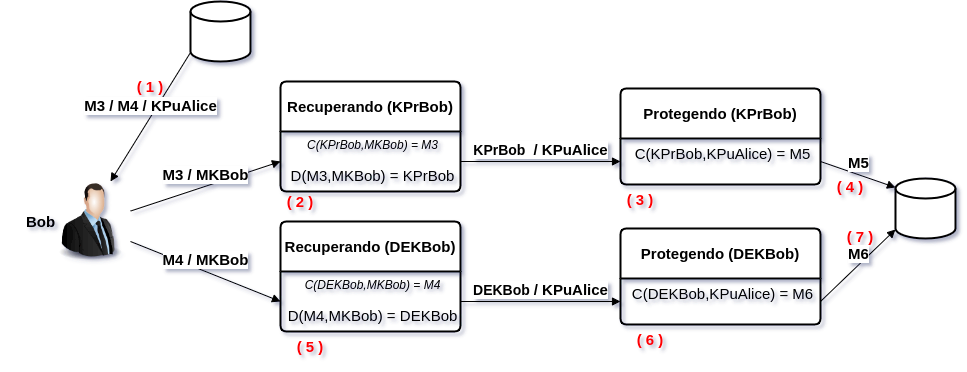
\includegraphics[scale=0.55]{custodiando.png}
	\caption{Processos de Custódia das Chaves do Bob}
	\label{fig:custodiando}
\end{figure}

\begin{enumerate}
	\item Bob recupera os Textos Cifrados M3 e M4 e a Chave Pública da Alice (KPuAlice.pem) do servidor;
	\item Bob descriptografa o Texto Cifrado M3 com sua Chave Mestra (MKBob.hex) e o IV associado para obter sua Chave Privada (KPrBob);
	\begin{tcolorbox}[width=\textwidth]
		{\scriptsize
			\begin{verbatim}
			$ openssl enc -d -aes-256-cbc -K "$(cat MKBob.hex)" -iv "$(cat M3.iv)" \
			  -in M3.bin -out KPrBob.pem
			\end{verbatim}
		}
	\end{tcolorbox}
	\item Bob protege a sua Chave Privada (KPrBob.pem) para a custodiante Alice, gerando o Texto Cifrado M5. O envelope CMS usa criptografia híbrida: cifra o conteúdo e encapsula a chave de conteúdo para o certificado da Alice (Alice.cert.pem).
	\begin{tcolorbox}[width=\textwidth]
		{\scriptsize
			\begin{verbatim}
			$ openssl cms -encrypt -binary -in KPrBob.pem -out M5.pem -outform PEM \
			  -recip Alice.cert.pem -aes256
			\end{verbatim}
		}
	\end{tcolorbox}
	\item Bob envia o Texto Cifrado M5 para o Servidor;
	\item Bob descriptografa o Texto Cifrado M4 com sua Chave Mestra (MKBob.hex) e o IV associado para obter sua Chave de Dados (DEKBob.bin);
	\begin{tcolorbox}[width=\textwidth]
		{\scriptsize
			\begin{verbatim}
			$ openssl enc -d -aes-256-cbc -K "$(cat MKBob.hex)" -iv "$(cat M4.iv)" \
			  -in M4.bin -out DEKBob.bin
			\end{verbatim}
		}
	\end{tcolorbox}
	\item Bob criptografa sua Chave de Dados (DEKBob.bin) com a Chave Pública da Alice (KPuAlice.pem), gerando o Texto Cifrado M6.bin;
	\begin{tcolorbox}[width=\textwidth]
		{\scriptsize
			\begin{verbatim}
			$ openssl pkeyutl -encrypt -inkey KPuAlice.pem -pubin -in DEKBob.bin -out M6.bin \
			  -pkeyopt rsa_padding_mode:oaep -pkeyopt rsa_oaep_md:sha256
			\end{verbatim}
		}
	\end{tcolorbox}	
	\item Bob envia o Texto Cifrado M6 para o Servidor;
\end{enumerate}

\pagebreak

% Página
\section{Recuperando Custódia das Chaves}

Em um cenário em que Bob perde sua Chave Mestra (MKBob.hex), ele solicita à custodiante Alice que criptografe suas duas chaves, Chave Privada (KPrBob.pem) e Chave de Dados (DEKBob.bin), com a Nova Chave Mestra (NMKBob.hex).

\subsection{Gerando Nova Chave Mestra - Bob}

\begin{figure}[H]
	\centering
	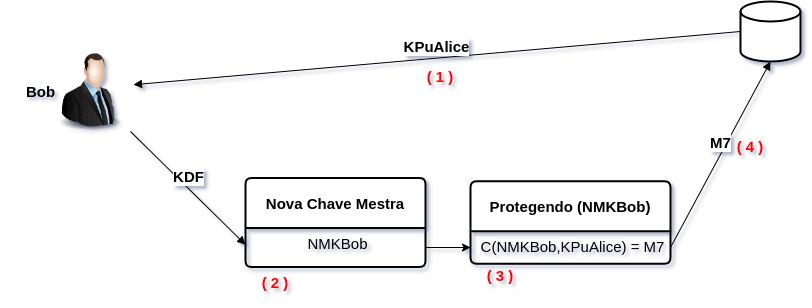
\includegraphics[scale=0.55]{nova-custodia_01.png}
	\caption{Processos de criação da Nova Chave Mestra do Bob}
	\label{fig:nova-custodia_01}
\end{figure}

\begin{enumerate}
	\item Bob recupera a Chave Pública da Alice (KPuAlice.pem) que está armazenada no servidor;
	\item Utilizando uma Key Derivation Function (KDF), Bob gera uma Nova Chave Mestra (NMKBob.hex);
	\begin{tcolorbox}[width=\textwidth]
		{\scriptsize
			\begin{verbatim}
				$ read -rs MASTER_PASSWORD
				$ SALT_HEX=$(openssl rand -hex 16)
				$ printf '%s' "$SALT_HEX" > NMKBob.salt
				$ openssl kdf -keylen 32 -kdfopt digest:SHA256 \
				  -kdfopt pass:"$MASTER_PASSWORD" -kdfopt salt:"$SALT_HEX" \
				  -kdfopt iter:600000 PBKDF2 | tr -d ':\n' > NMKBob.hex
			\end{verbatim}
		}
	\end{tcolorbox}
	\item Utilizando a Chave Pública da Alice (KPuAlice.pem), Bob protege sua Nova Chave Mestra (NMKBob.hex), gerando o Texto Cifrado M7;
	\begin{tcolorbox}[width=\textwidth]
		{\scriptsize
			\begin{verbatim}
			$ openssl pkeyutl -encrypt -inkey KPuAlice.pem -pubin -in NMKBob.hex -out M7.bin \
			  -pkeyopt rsa_padding_mode:oaep -pkeyopt rsa_oaep_md:sha256
			\end{verbatim}
		}
	\end{tcolorbox}
	\item O Texto Cifrado M7 é enviado para o servidor.
\end{enumerate}

\subsection{Nova Custódia - Alice}

\begin{figure}[H]
	\centering
	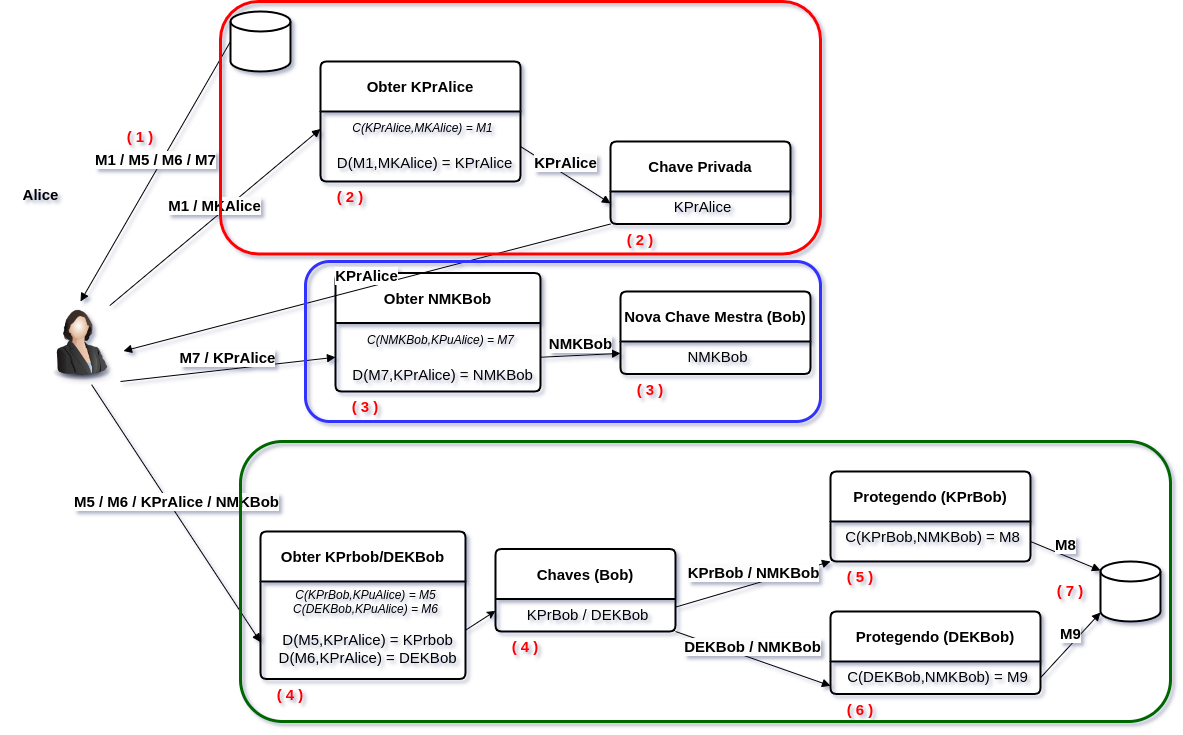
\includegraphics[scale=0.45]{nova-custodia_02.png}
	\caption{Processos de proteção das chaves do Bob com a sua Nova Chave Mestra}
	\label{fig:nova-custodia_02}
\end{figure}

\begin{enumerate}
	\item Alice faz o download dos Textos Cifrados M1, M5, M6 e M7 do servidor;
	\item Alice descriptografa o Texto Cifrado M1 com sua Chave Mestra (MKAlice.hex) e o IV associado para obter sua Chave Privada (KPrAlice.pem);
	\begin{tcolorbox}[width=\textwidth]
		{\scriptsize
			\begin{verbatim}
			$ openssl enc -d -aes-256-cbc -K "$(cat MKAlice.hex)" -iv "$(cat M1.iv)" \
			  -in M1.bin -out KPrAlice.pem
			\end{verbatim}
		}
	\end{tcolorbox}
	\item Com sua Chave Privada (KPrAlice.pem), Alice descriptografa o Texto Cifrado M7 e obtém a Nova Chave Mestra (NMKBob.hex) do Bob;
	\begin{tcolorbox}[width=\textwidth]
		{\scriptsize
			\begin{verbatim}
			$ openssl pkeyutl -decrypt -inkey KPrAlice.pem -in M7.bin -out NMKBob.hex \
			  -pkeyopt rsa_padding_mode:oaep -pkeyopt rsa_oaep_md:sha256
			\end{verbatim}
		}
	\end{tcolorbox}
	\item Com sua Chave Privada (KPrAlice.pem), Alice recupera os artefatos de custódia M5 e M6 e obtém a Chave Privada do Bob (KPrBob.pem) e a Chave de Dados do Bob (DEKBob.bin);
	\begin{tcolorbox}[width=\textwidth]
		{\scriptsize
			\begin{verbatim}
			  -inkey KPrAlice.pem -out KPrBob.pem
			$ openssl cms -decrypt -in M5.pem -inform PEM -recip Alice.cert.pem \
			  -inkey KPrAlice.pem -out KPrBob.pem
			  -inkey KPrAlice.pem -out KPrBob.pem

			$ openssl pkeyutl -decrypt -inkey KPrAlice.pem -in M6.bin -out DEKBob.bin \
			  -pkeyopt rsa_padding_mode:oaep -pkeyopt rsa_oaep_md:sha256
			\end{verbatim}
		}
	\end{tcolorbox}
	\item Com a Nova Chave Mestra do Bob (NMKBob.hex), Alice criptografa a Chave Privada do Bob (KPrBob.pem) gerando o Texto Cifrado M8;
	\begin{tcolorbox}[width=\textwidth]
		{\scriptsize
			\begin{verbatim}
			$ IV_HEX=$(openssl rand -hex 16)
			$ printf '%s' "$IV_HEX" > M8.iv
			$ openssl enc -aes-256-cbc -K "$(cat NMKBob.hex)" -iv "$IV_HEX" \
			  -in KPrBob.pem -out M8.bin
			\end{verbatim}
		}
	\end{tcolorbox}
	\item Com a Nova Chave Mestra do Bob (NMKBob.hex), Alice criptografa a Chave de Dados do Bob (DEKBob.bin) gerando o Texto Cifrado M9;
	\begin{tcolorbox}[width=\textwidth]
		{\scriptsize
			\begin{verbatim}
			$ IV_HEX=$(openssl rand -hex 16)
			$ printf '%s' "$IV_HEX" > M9.iv
			$ openssl enc -aes-256-cbc -K "$(cat NMKBob.hex)" -iv "$IV_HEX" \
			  -in DEKBob.bin -out M9.bin
			\end{verbatim}
		}
	\end{tcolorbox}
	\item Os Textos Cifrados M8 e M9 são enviados para o servidor.
\end{enumerate}

A partir deste ponto, a Chave Privada do Bob (KPrBob.pem) e a Chave de Dados do Bob (DEKBob.bin) estão protegidas com a Nova Chave Mestra do Bob (NMKBob.hex) e estão armazenadas no servidor. Os IVs M8.iv e M9.iv acompanham os respectivos textos cifrados.

\pagebreak

%Copyright
\vspace*{\fill}
\begin{flushright}
	\underline{\textit{Copyright}}\\
	All rights reserved to MT4 Tecnologia LTDA.\bigskip

	\underline{\textit{Propósito deste documento}}\\
	New MySafe - Account Recovery\bigskip

	\underline{\textit{Versão}}\\
	Versão 1.0\bigskip

	\underline{\textit{Autor}}\\
	Caio Abreu Ferreira [\href{mailto:cferreira@senhasegura.com}{cferreiras@senhasegura.com}] \bigskip\\
	
	\underline{\textit{MT4 Tecnologia Ltda.}}\\
	Rua Joaquim Antunes, 767 – Pinheiros – São Paulo\\
	Phone: +55 11 3065-7070\\
	\url{www.mt4.com.br}\\
\end{flushright}

\end{document}
